\subsection{Logarithms}\label{sec:logarithm}
\subsubsection{Introduction}
You are already familiar with the concept of \textit{exponentiation}, which means raising a number to an exponent. Take for example $16=2^4$. Here, $2$ is called the \textit{base} and $4$ is called the \textit{exponent} or \textit{power}.

The \textit{logarithm}, first introduced by \textit{John Napier} in $1614$, is the inverse operation of exponentiation. For instance, the logarithm of $64$ in base $2$ is $6$ because $64=2^6$.

\begin{definition}
	Let $x$ and $b$ be positive real numbers such that $b \neq 1$. The logarithm of $x$ to base $b$ is the exponent by which $b$ must be raised to yield $x$.  In other words, the logarithm of $x$ to base $b$ is the solution $y$ to the equation
	\begin{align*}
		b^y = x
	\end{align*}
	We denote this by $y = \log_b x$.
\end{definition}

\begin{remark}
	$ $
	\begin{enumerate}
		\item The base of the logarithm cannot be equal to $1$. The reason is simple: the equation $1^x = 1^y$ holds for all the values of $x$ and $y$, and the definition of logarithm to base $1$ would be pointless\watermark.

		\item Some books use the notation $\log x$ (no base presented) to mean \textit{common logarithm}\footnote{or decimal logarithm.}. That is, logarithm to base $10$. For example, $\log 1000=3$.

		\item The logarithm to the base of mathematical constant $e$ is called the \textit{natural logarithm}.\footnote{$e\approx 2.71828.$} The natural logarithm of $x$ is generally written as $\ln x$.
	\end{enumerate}
\end{remark}

\begin{example}
	$ $
	\begin{enumerate}
		\item Let $a \neq 1$ be a positive real number. Then $\log_a a=1$ and $\log_a 1 = 0$.
		\item $\log_5 \dfrac{1}{125}=-3$.
		\item $\log_{1/7} 49 = -2$.
		\item $\log_{49} \sqrt 7 = 0.25$.
		\item $\log 0.0001 = -4$.
	\end{enumerate}
\end{example}
\subsubsection{Laws of Logarithms}


As in exponentiation where you can write $a^x \cdot a^y = a^{x+y}$, a similar relation for logarithms can be written. This, along with a few other properties of logarithms, are introduced in the following proposition.

\begin{proposition}[Laws of Logarithms]\label{prop:log_laws}
	Let $a$ and $b$ be positive reals not equal to $1$. For any two positive reals $x$ and $y$, we have
	\begin{enumerate}
		\item $\log_a xy = \log_a x + \log_a y$.
		\item $\log_a \dfrac{x}{y} = \log_a x - \log_a y$.
		\item $\log_{a^n} x^m = \dfrac{m}{n}\log_a x$ for any real $m$ and $n$ (with $n \neq 0$).
		\item $\log_a b = \dfrac{1}{\log_b a}$.
		\item $\log_a x = \dfrac{\log_b x}{\log_b a}$.
	\end{enumerate}
\end{proposition}

\begin{proof}
	The proofs are rather straightforward. We prove the first and the last parts and leave others as exercises for the reader. For the first part, let $\log_a x= m$ and $\log_a y =n$. Then by definition, $x=a^m$ and $y=a^n$. Thus,
	\begin{align*}
		xy=a^{m+n}
	\end{align*}
	which in turn gives $\log_a xy = m+n$. For the last part, assume $\log_b x = m$ and $\log_b a=n$. Then $x=b^m$ and $a=b^n$ and so by part $3$,
	\begin{align*}
		\log_a x
		& = \log_{b^n} b^m\\
		& = \frac{m}{n} \log_b b =\frac{m}{n} \\
		& =\dfrac{\log_b x}{\log_b a}
	\end{align*}
	since $\log_b b =1$.
\end{proof}

\begin{note}
	Both $\log_a (x+y) = \log_a x + \log_a y$ and $\log_a (x+y) = \log_a x \cdot \log_a y$ are \textbf{false}. Do not use them.
\end{note}

\begin{example}
	Suppose that you know the logarithm of every number to base $e$. How would you find $\log_3 5$? The answer would be to use the last part of proposition \eqref{prop:log_laws}:
	\begin{align*}
		\log_3 5
		& = \frac{\ln 5}{\ln 3}\\
		& \approx \frac{1.6094}{1.0986}\\
		& \approx 1.4649
	\end{align*}
	You can easily find the values of $\ln 5$ and $\ln 3$ using a simple scientific calculator.
\end{example}

\begin{example}
	Given that $\log_2 3 \approx 1.5849$, let's find $\log_{0.125} 36$. Notice that $0.125=1/8=2^{-3}$ and $36=2^2 \cdot 3^2$. Therefore,
	\begin{align*}
		\log_{0.125} 36
		&= \log_{2^{-3}} \left(2^2 \cdot 3^2\right)\\
		& = \log_{2^{-3}} 2^2 + \log_{2^{-3}} 3^2\\
		& = \frac{2}{-3} \log_2 2 + \frac{2}{-3} \log_2 3\\
		& \approx -\frac{2}{3}(1+1.5849)\\
		& \approx -1.7232
	\end{align*}
\end{example}

\begin{figure}[t]
	\centering
	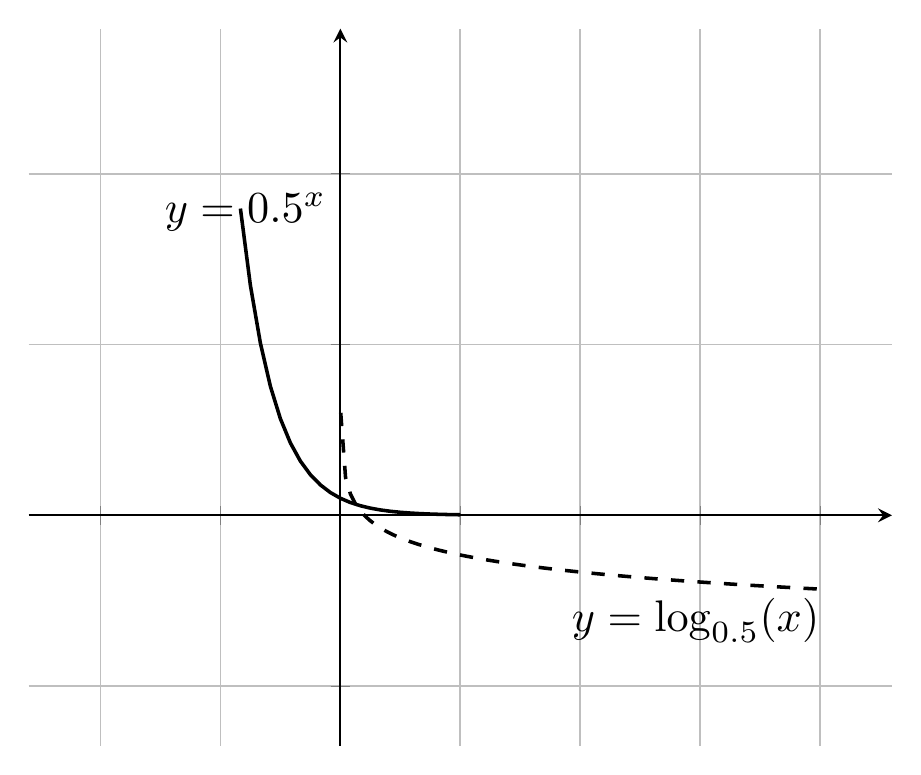
\begin{tikzpicture}[scale = 1.6]
		\begin{axis}[grid=both,
			xmin=-10,xmax=20,ymin=-10,ymax=25,
			yticklabels={,,},
			xticklabels={,,},
			axis lines=middle,
			restrict y to domain=-15:21,
			enlargelimits]
			\addplot[, thick]  {pow(0.5,x)} node[pos=0.1, above]{$y=0.5^x$};
			\addplot[,domain=1/2^6:20,samples=100, thick, dashed]  {ln(x)/ln(0.5)} node[pos=0.8,below] {$y=\log_{0.5}(x)$};
		\end{axis}
	\end{tikzpicture}
	\caption{Plot of functions $y=\log_{0.5} x$ and $y=0.5^x$.}
	\label{fig:log_exp_0.5}
\end{figure}

\begin{proposition}\label{prop:log_strict}
	Let $b, x_1, x_2$ be positive real numbers such that $b\neq 1$. Then
	\begin{enumerate}
		\item if $b>1$, $x_1>x_2$ if and only if $\log_b x_1 > \log_b x_2$,
		\item if $b<1$, $x_1>x_2$ if and only if $\log_b x_1 < \log_b x_2$.
	\end{enumerate}
\end{proposition}

\begin{proof}
	We illustrate the proof with two sample cases. In Figure \ref{fig:log_exp_2}, you can see the plot of $y=\log_2 x$ for $x \in [0, 10]$. As seen in the figure, logarithm to the base $2$ is strictly increasing. That is, if $x_1>x_2$, then $\log_2 x_1 > \log_2 x_2$. Now, let's prove that if $\log_2 x_1 > \log_2 x_2$, then $x_1>x_2$. In the same figure, you can see the plot of $y=2^x$, which is, again, strictly increasing. It means that for any two reals $x_1$ and $x_2$, if $x_1>x_2$, then $2^{x_1} > 2^{x_2}$. By definition, we can find positive reals $y_1$ and $y_2$ such that $x_1 = \log_2 y_1$ and $x_2=\log_2 y_2$. Now, the relation
	\begin{align*}
		x_1>x_2 \implies 2^{x_1} > 2^{x_2}
	\end{align*}
	transforms to
	\begin{align*}
		\log_2 y_1
		& > \log_2 y_2\\
		\implies y_1
		& > y_2
	\end{align*}
	which is what we wanted. Analogously, as shown in Figure \ref{fig:log_exp_0.5}, the functions $y=\log_{0.5} x$ and $y=0.5^x$ are both strictly decreasing and the proof of part $2$ is almost the same as the previous part.
\end{proof}

\begin{figure}[t]
	\centering
	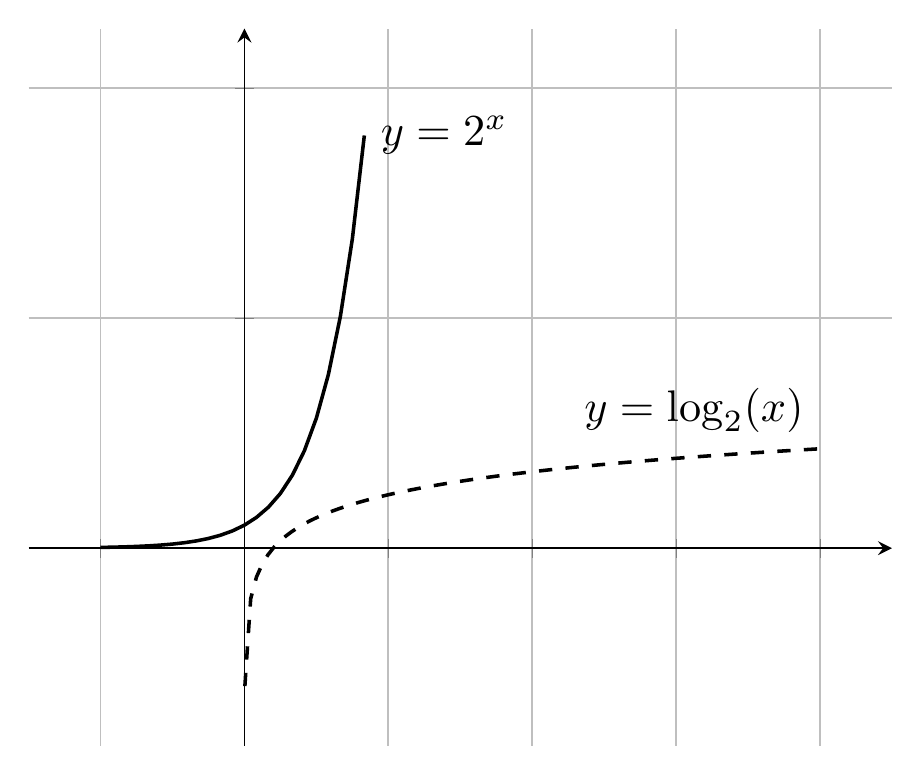
\begin{tikzpicture}[scale = 1.6]
		\begin{axis}[grid=both,
			xmax=20,ymax=20,
			yticklabels={,,},
			xticklabels={,,},
			axis lines=middle,
			restrict y to domain=-7:21,
			enlargelimits]
			\addplot[, thick]  {pow(2,x)} node[right]{$y=2^x$};
			\addplot[,domain=1/2^6:20,samples=100,thick, dashed]  {ln(x)/ln(2)} node[above left] {$y=\log_2(x)$};
		\end{axis}
	\end{tikzpicture}
	\caption{Plot of functions $y=\log_2 x$ and $y=2^x$.}
	\label{fig:log_exp_2}
\end{figure}